\documentclass{beamer}
\usepackage{beamerthemeshadow}
\usepackage{graphicx}
\usepackage[absolute,overlay]{textpos}
\begin{document}
\title{Version control with git}
\author{Eike Mueller, University of Bath}
\date{Thu $27^{\text{th}}$ Sep 2018} 

%%%%%%%%%%%%%%%%%%%%%%%%%%%%%%%%%%%%%%%%%%%%%%%%%%%%%%%%%%%%%%%%%%%%%%

\begin{frame}
  \frametitle{$ $}
  \titlepage
\end{frame}

%%%%%%%%%%%%%%%%%%%%%%%%%%%%%%%%%%%%%%%%%%%%%%%%%%%%%%%%%%%%%%%%%%%%%%

\begin{frame}
  \frametitle{Why version control?}
  \begin{center}
    
\includegraphics[width=0.5\linewidth]{phdcomics.png}
  \end{center}
  {\footnotesize ``Piled Higher and Deeper'' by Jorge Cham, \texttt{http://www.phdcomics.com}}
\end{frame}

%%%%%%%%%%%%%%%%%%%%%%%%%%%%%%%%%%%%%%%%%%%%%%%%%%%%%%%%%%%%%%%%%%%%%%

\begin{frame}
  \frametitle{Version control}
  \textbf{\Large Benefits of Version control}
  \begin{itemize}
  \item Systematic and controlled \textbf{Backup}
  \item \textbf{Collaborate}: work on same document simultaneously
  \item Keep \textbf{track} of \textbf{changes} (who introduced feature X and why?)
  \item \textbf{Try out changes} and \textbf{revert} to working version (``undo''-button)
  \item Work on project on \textbf{different machines}
  \item Simplifies \textbf{debugging}
  \item \textbf{Reproducibility}
  \end{itemize}
  \vspace{2ex}
  \textbf{\Large What's the catch?}
  \begin{itemize}
    \item Have to learn a few commands to interact with git
    \item Enforces organised approach
  \end{itemize}
  \begin{textblock}{1.0}(11,8)
    
\includegraphics[width=3.5cm]{bughunting.png}
  \end{textblock}
\end{frame}

%%%%%%%%%%%%%%%%%%%%%%%%%%%%%%%%%%%%%%%%%%%%%%%%%%%%%%%%%%%%%%%%%%%%%%

\begin{frame}
  \frametitle{Applications}
  \textbf{\Large Version control can be be applied to:}
  \begin{itemize}
  \item \textbf{Source code} (matlab, Fortran, C, Python, \dots)
  \item \textbf{LaTeX} (papers, reports, your thesis, \dots)
  \item Raw \textbf{results} (e.g. CSV files with numerical values)
  \item \textbf{Any text} files\footnotemark
  \end{itemize}
  \vspace{4ex}
  \textbf{\Large Reproducibility:}
  Link results to particular code version
  \footnotetext{Binary files work as well, but harder to track changes}
\end{frame}

%%%%%%%%%%%%%%%%%%%%%%%%%%%%%%%%%%%%%%%%%%%%%%%%%%%%%%%%%%%%%%%%%%%%%%

\begin{frame}
  \frametitle{Basic concepts}
  \begin{center}
    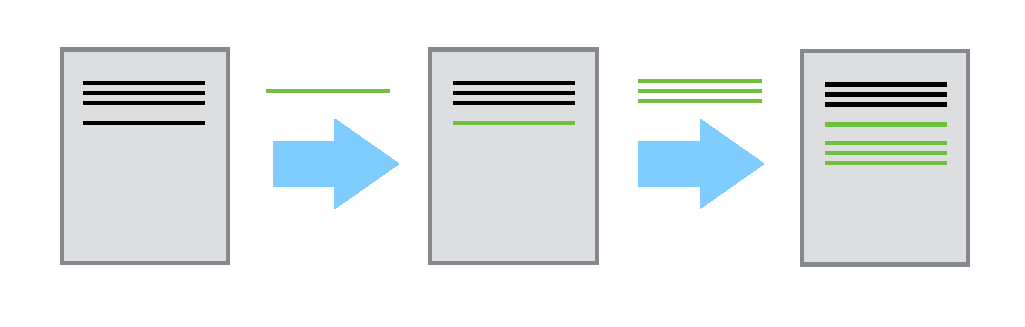
\includegraphics[width=0.6\linewidth]{play-changes.pdf}\\
    Tracking of changes
  \end{center}
  \begin{minipage}{0.45\linewidth}
    \begin{center}
      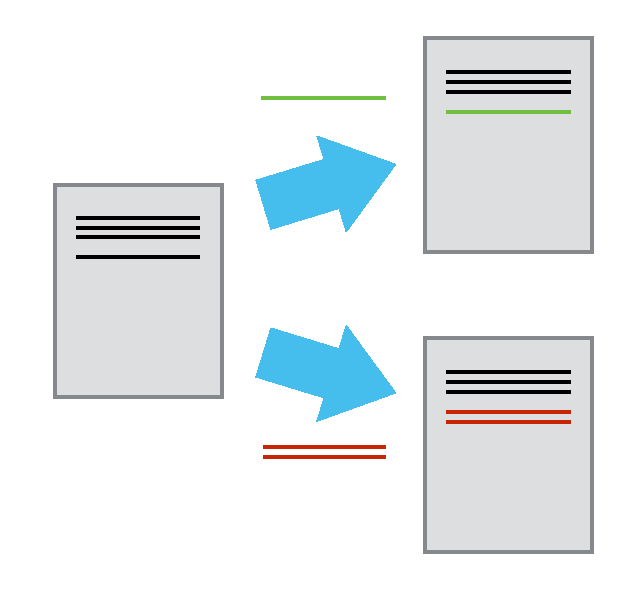
\includegraphics[width=0.6\linewidth]{versions.pdf}\\
      Collaborating
    \end{center}
  \end{minipage}
  \begin{minipage}{0.45\linewidth}
    \begin{center}
      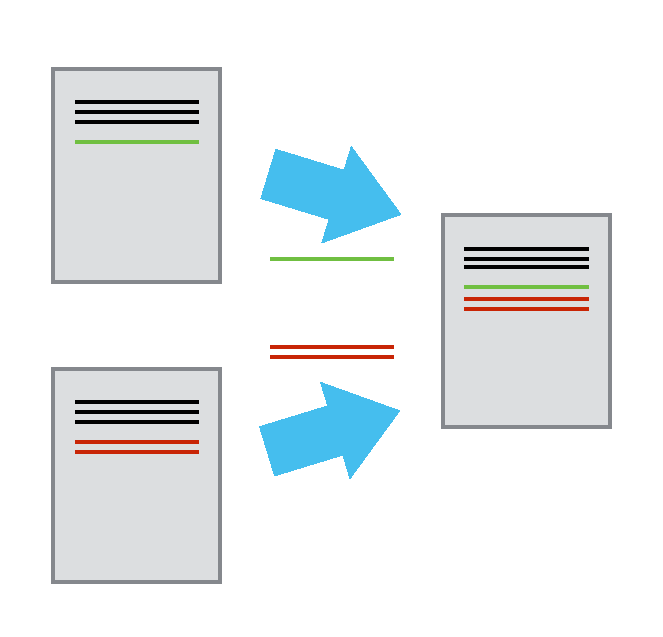
\includegraphics[width=0.6\linewidth]{merge.pdf}\\
      Merging and resolving conflicts
    \end{center}
  \end{minipage}\\[2ex]
  {\footnotesize All figures from Software Carpentry webpage}
\end{frame}

%%%%%%%%%%%%%%%%%%%%%%%%%%%%%%%%%%%%%%%%%%%%%%%%%%%%%%%%%%%%%%%%%%%%%%

\begin{frame}
  \frametitle{git}
  \textbf{\Large Why git?}
  \begin{itemize}
  \item \textbf{de-facto} standard now (supersedes subversion, CVS, \dots)
  \item Several nice features:
    \begin{itemize}
      \item Work remotely (distributed system allows \textbf{offline commits})
      \item Simple and lightweight \textbf{branching}\\$\Rightarrow$ encourages experimentation
      \item Selective commits (\textbf{staging} area)
      \item Very \textbf{powerful}
    \end{itemize}
  \item Not the easiest system to learn
    \begin{itemize}
      \item We'll only cover the basics here
      \item Lots of online resources
      \item Graphical interfaces (e.g. SourceTree)
    \end{itemize}
  \end{itemize}
  \vspace{2ex}
  \textbf{\Large Documentation}
  \begin{itemize}
  \item Git book: \texttt{http://git-scm.com/book/en/v2}
  \item Reference: \texttt{http://git-scm.com/docs}
  \end{itemize}
\end{frame}

%%%%%%%%%%%%%%%%%%%%%%%%%%%%%%%%%%%%%%%%%%%%%%%%%%%%%%%%%%%%%%%%%%%%%%

\begin{frame}
  \frametitle{Overview}
  \textbf{\Large Session 1} (Basics) {\color{red}{13:45h - 15:00h}}
  \begin{itemize}
  \item Creating a git repository
  \item Tracking changes
  \item Exploring history
  \end{itemize}
  \vspace{-1ex}
  \begin{center}
  --- break ---
  \end{center}
  \vspace{-1ex}
  \textbf{\Large Session 2} (Collaborating) {\color{red}{15:30h - 17:00h}}
  \begin{itemize}
  \item Working with remotes (github)
  \item Collaborating and resolving conflicts
  \item Wrapup and advanced concepts (branching, merging, \dots)
  \end{itemize}
  \vspace{1ex}
  Resources available at\footnote{All material used is based on Software Carpentry webpage \texttt{http://software-carpentry.org/}}
 \texttt{http://people.bath.ac.uk/rjg20/training/}
\end{frame}

%%%%%%%%%%%%%%%%%%%%%%%%%%%%%%%%%%%%%%%%%%%%%%%%%%%%%%%%%%%%%%%%%%%%%%

\begin{frame}
  \frametitle{${}^{}$}
\end{frame}

%%%%%%%%%%%%%%%%%%%%%%%%%%%%%%%%%%%%%%%%%%%%%%%%%%%%%%%%%%%%%%%%%%%%%%

\begin{frame}
  \frametitle{github}
  \textbf{Create a github account}
  \begin{center}
    go to {\color{blue}{\texttt{https://github.com/}}}
  \end{center}
  \begin{center}
    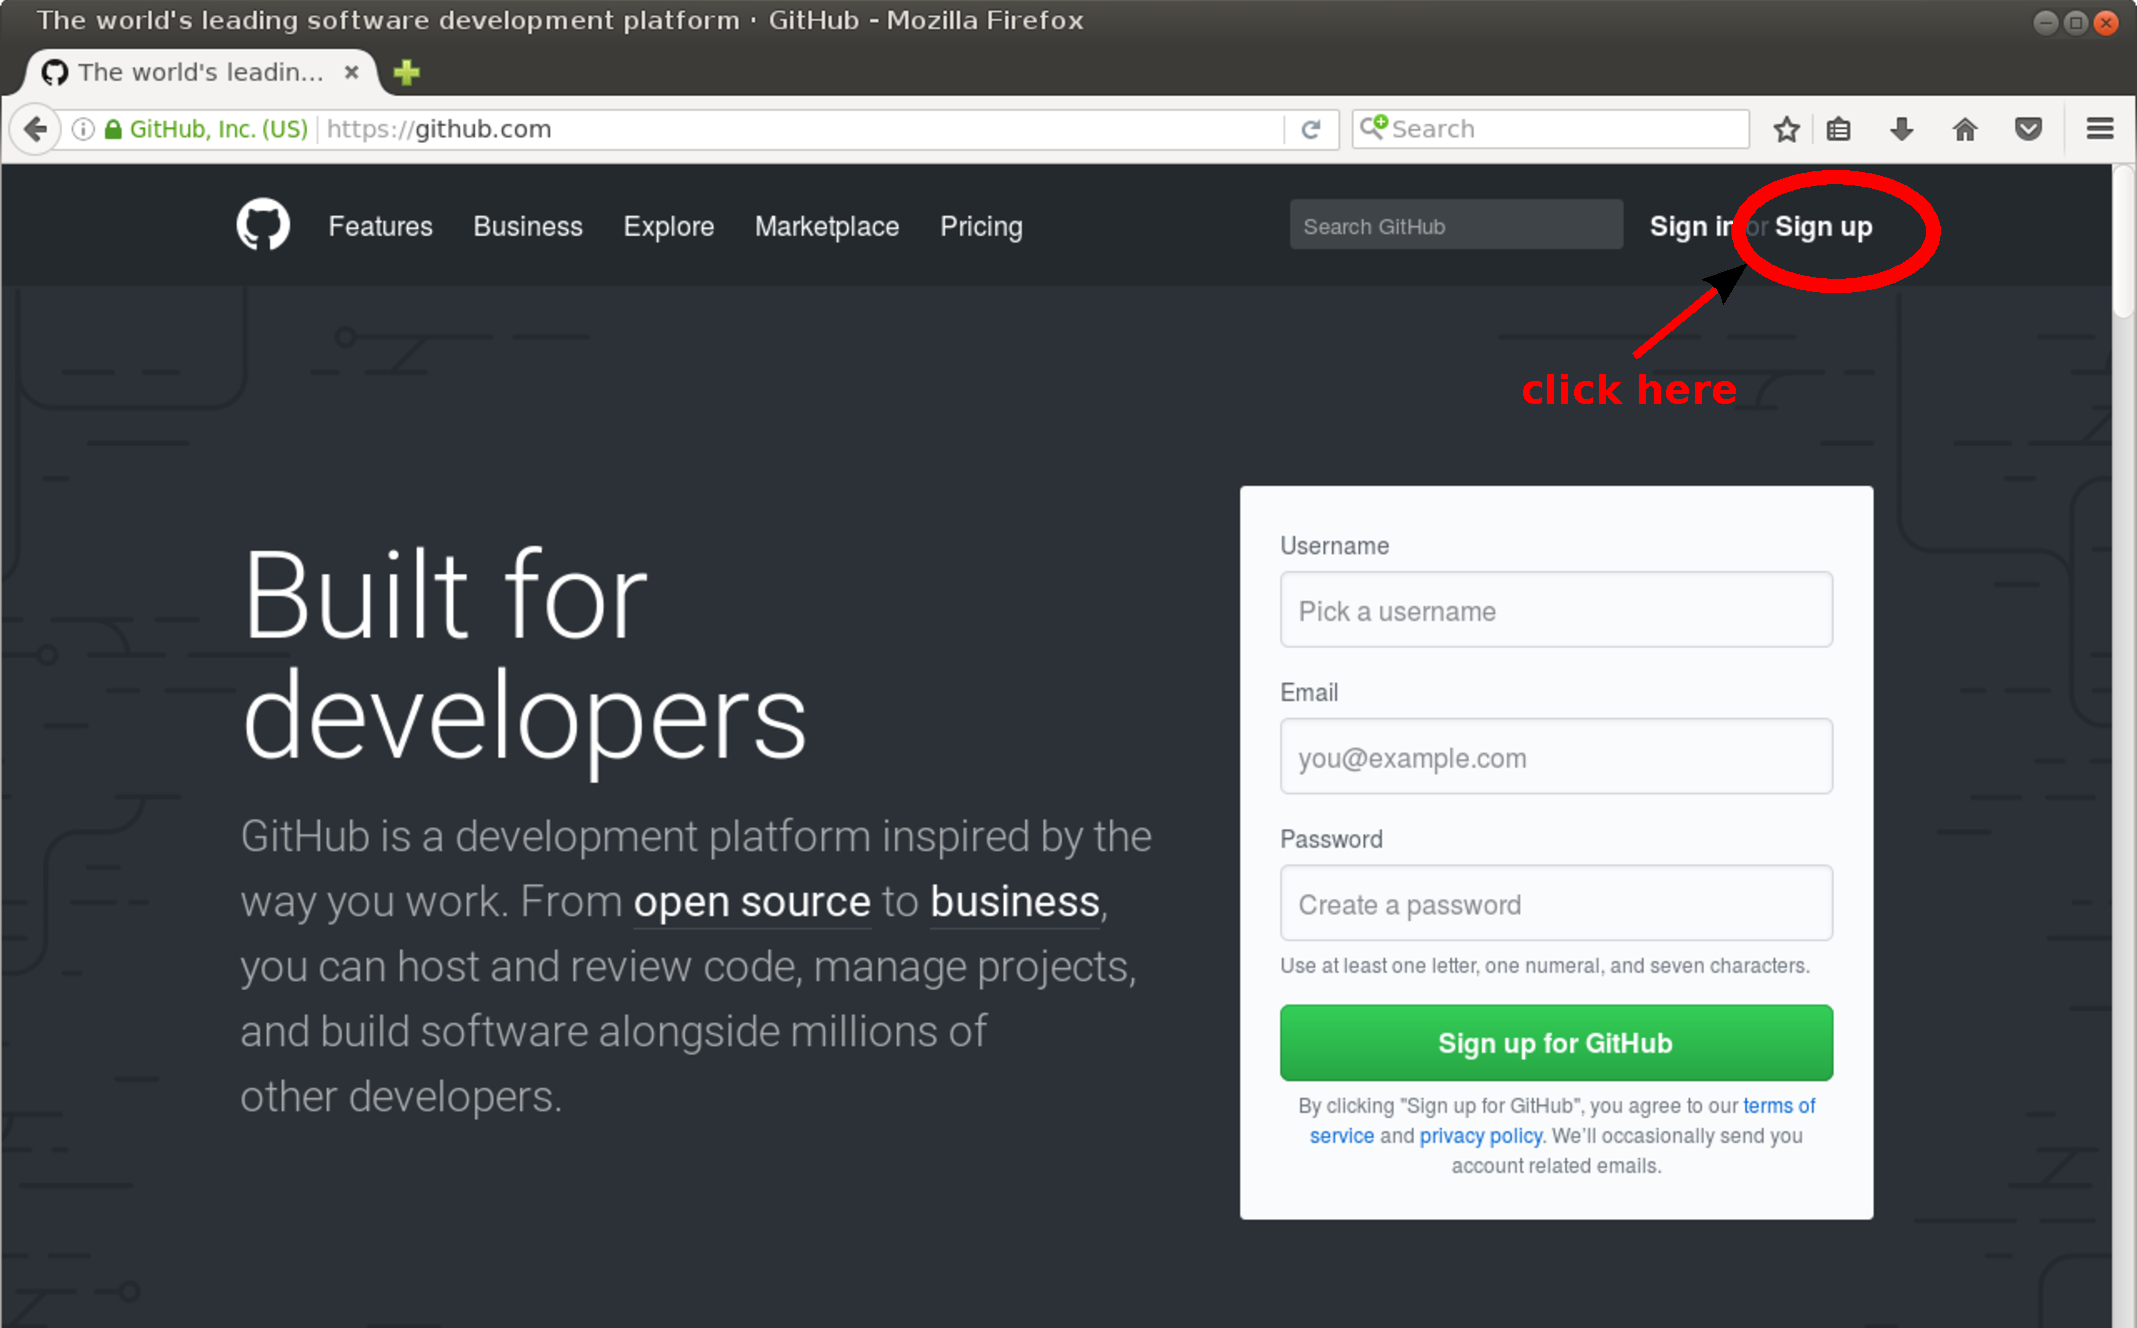
\includegraphics[width=0.75\linewidth]{github.pdf}
  \end{center}
  Use your \underline{University email address}
\end{frame}

%%%%%%%%%%%%%%%%%%%%%%%%%%%%%%%%%%%%%%%%%%%%%%%%%%%%%%%%%%%%%%%%%%%%%%

\begin{frame}
  \frametitle{${}^{}$}
\end{frame}

%%%%%%%%%%%%%%%%%%%%%%%%%%%%%%%%%%%%%%%%%%%%%%%%%%%%%%%%%%%%%%%%%%%%%%

\begin{frame}
  \frametitle{Wrapup}
  \textbf{\Large Summary}
  \begin{itemize}
    \item Track changes and collaborate
    \item Pays off even for small projects
    \item Small number of commands
      \begin{enumerate}
        \item \texttt{git log}
        \item \texttt{git status}
        \item \texttt{git add}
        \item \texttt{git commit}
        \item \texttt{git clone/push/pull}
      \end{enumerate}
    \item There are \textbf{graphical tools} (e.g. SourceTree for Mac/Win)
    \item Other hosting sites: BitBucket, GitLab
  \end{itemize}
  \textbf{\Large More details}
  \begin{itemize}
  \item Git book: \texttt{http://git-scm.com/book/en/v2}
  \item Reference: \texttt{http://git-scm.com/docs}
  \end{itemize}
\end{frame}

%%%%%%%%%%%%%%%%%%%%%%%%%%%%%%%%%%%%%%%%%%%%%%%%%%%%%%%%%%%%%%%%%%%%%%

\begin{frame}
  \frametitle{Advanced topics}
  \textbf{\Large Advanced topics}
  \begin{itemize}
    \item What actually is a commit?
    \item Branching and merging, the \texttt{rebase} command
    \item Rewriting history
    \item Pull requests
    \item Advanced workflows
    \item Forking repositories
    \item Tags
    \item Stashing
  \end{itemize}
\end{frame}

%%%%%%%%%%%%%%%%%%%%%%%%%%%%%%%%%%%%%%%%%%%%%%%%%%%%%%%%%%%%%%%%%%%%%%

\begin{frame}
  \frametitle{Branches}
  \textbf{\Large A Quick glance at branches}\\[1ex]
  Branches allow organised simultaneous development by collecting related 
  commits\\
  \begin{minipage}{0.45\linewidth}
  \begin{itemize}
    \item Bugfix
    \item New untested feature
    \item Master branch (guaranteed to work)
  \end{itemize}
  Usually:
  \begin{equation*}
    \text{\textbf{1 concept/feature}} = \text{\textbf{1 branch}}
  \end{equation*}
  \end{minipage}
  \hfill
  \begin{minipage}{0.45\linewidth}
  \begin{center}
    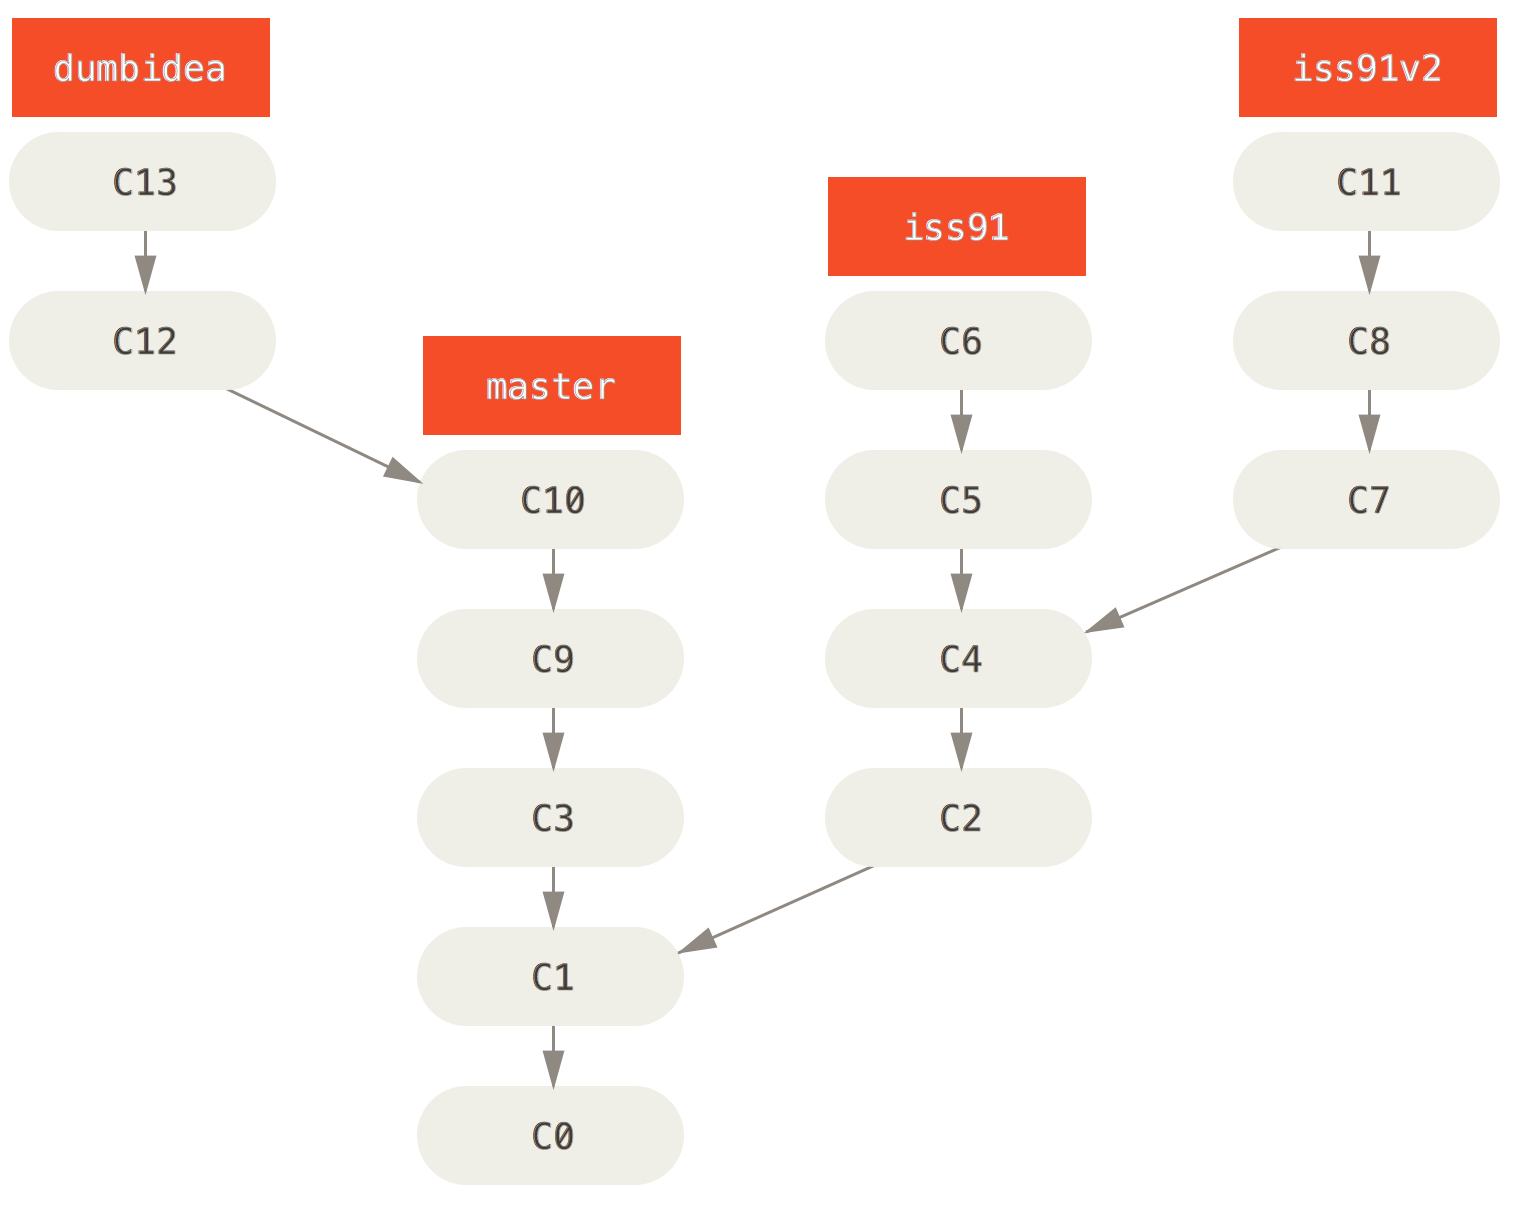
\includegraphics[width=0.95\linewidth]{topic-branches-1.png}
  \end{center}
  {\footnotesize \texttt{https://git-scm.com/book}}
  \end{minipage}\\[2ex]
  git branch = \textbf{lightweight} pointer
\end{frame}

%%%%%%%%%%%%%%%%%%%%%%%%%%%%%%%%%%%%%%%%%%%%%%%%%%%%%%%%%%%%%%%%%%%%%%

\begin{frame}
  \frametitle{Branches}
  \textbf{\Large Merge and resolve conflicts}\\[1ex]
  \begin{itemize}
    \item Basic merge and rebase
    \item Pull requests on github and BitBucket
    \item Code review
    \item Can limit access to master branch
  \end{itemize}
  \begin{center}
    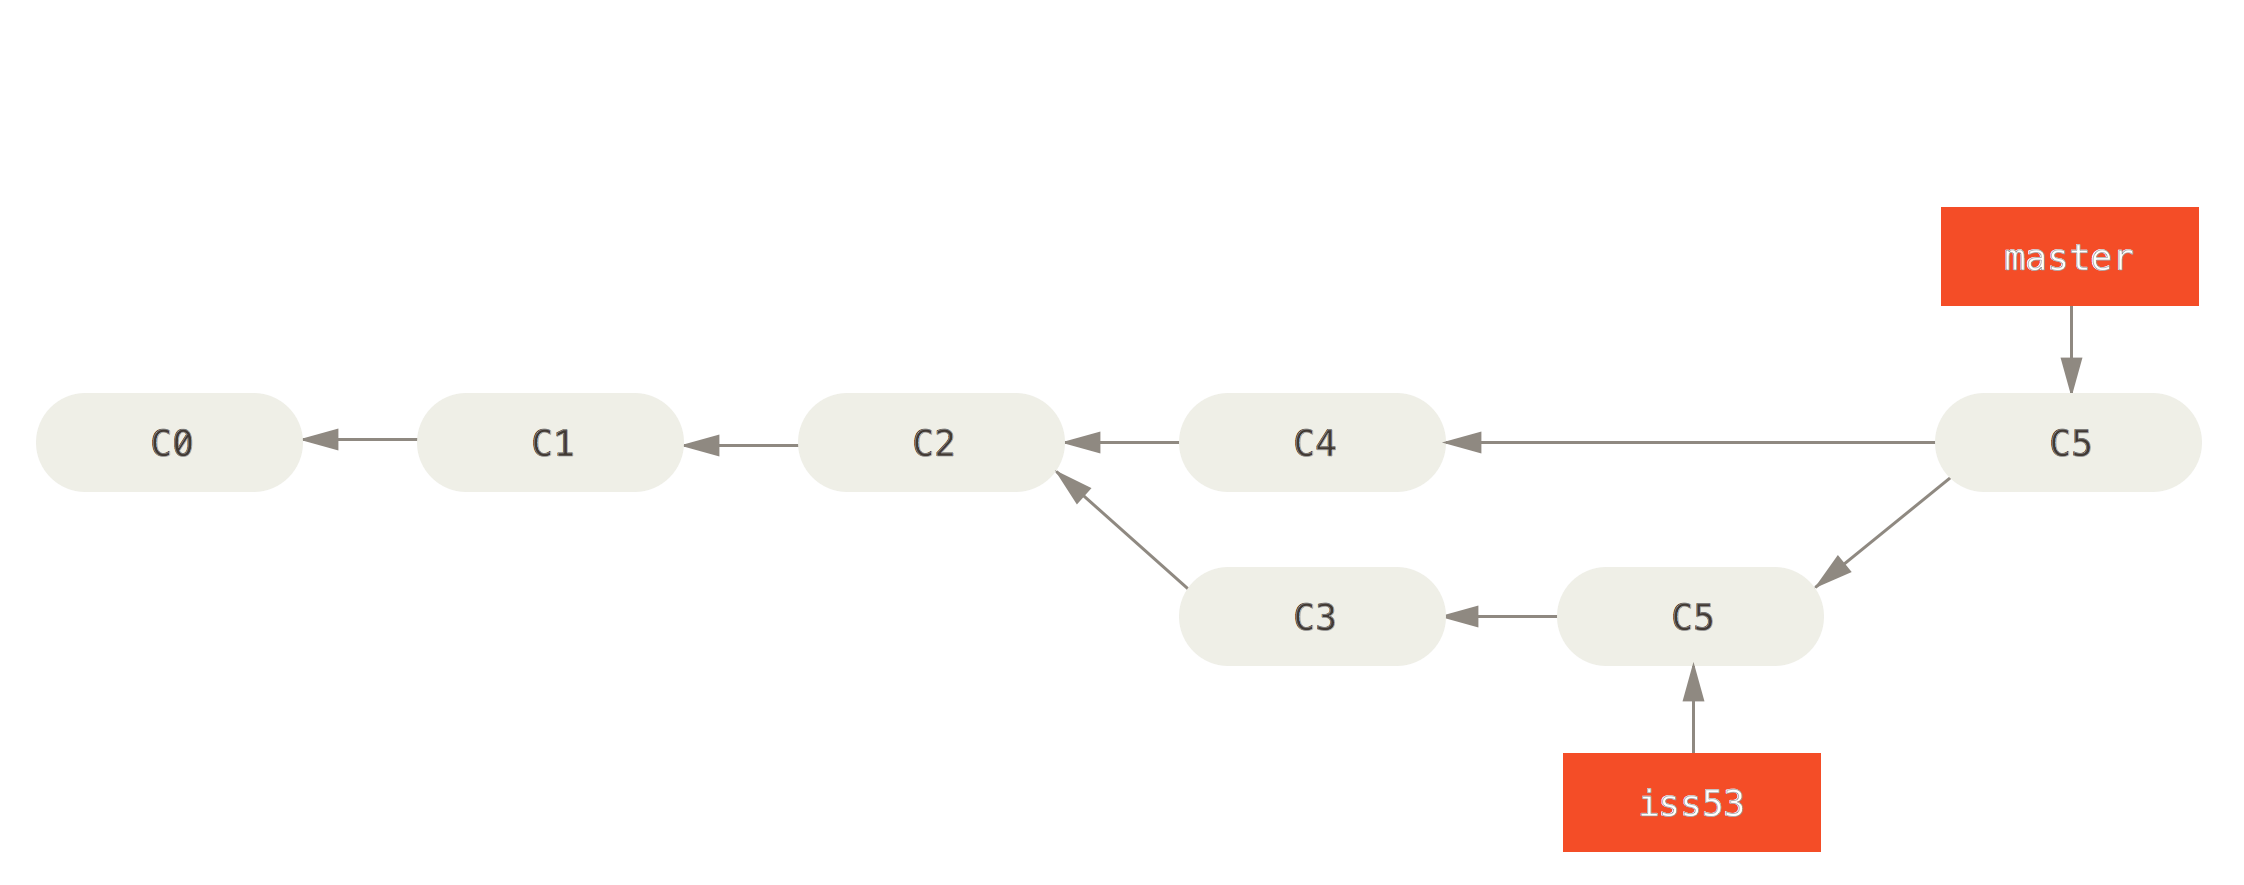
\includegraphics[width=0.9\linewidth]{basic-merging-2.png}\\
    {\footnotesize \texttt{https://git-scm.com/book}}
  \end{center}
\end{frame}

\end{document}
